%!TEX root = ../report.tex

\section{Approach}
\label{sec:approach}
We propose a modular framework for transfer learning in reinforcement learning. 
The framework consists of three modules: 
i) the \textbf{representation module}, which constructs an abstract representation of the task environment;
ii) the \textbf{policy learner}, which is a RL learner operating based on the task abstraction created by the representation module;
iii) the \textbf{task environment}, which is the RL task to be solved by the policy learner.

\subsection{Representation Module}
The representation module aims to construct an abstract and generalized representation of the environment's states to facilitate later knowledge transfer.
In this work, several architectures are proposed as visualized in Figure \ref{fig:repr_learner}.
These architectures all include some lower-dimensional ``bottleneck'' layers for dimensionality reduction of the input.
Once learned, this intermediate latent space is expected to create a more compact and abstract representation of the original environment and serve as the basis of transfer learning. 

\begin{figure}[ht!]
	\centering
	\begin{subfigure}{0.45\columnwidth}
		\centering
		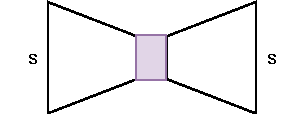
\includegraphics[width=\linewidth]{img/very_simple_autoencoder.pdf}
		\caption{Simple autoencoder}
		\label{subfig:repr_learner_simple_autoencoder}
	\end{subfigure}%
	~ 
	\begin{subfigure}{0.45\columnwidth}
		\centering
		\includegraphics[width=\linewidth]{documentation/report/img/variational_autoencoder_ver2.png}
		\caption{Variational autoencoder}
		\label{subfig:repr_learner_vae}
	\end{subfigure}
	\begin{subfigure}{0.5\columnwidth}
		\centering
		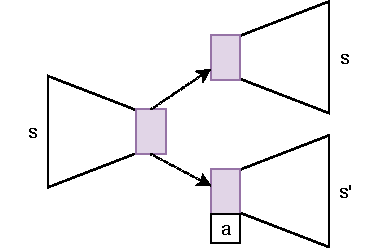
\includegraphics[width=\linewidth]{img/janus.pdf}
		\caption{Janus}
		\label{subfig:repr_learner_janus}
	\end{subfigure}%
	~ 
	\begin{subfigure}{0.5\columnwidth}
		\centering
		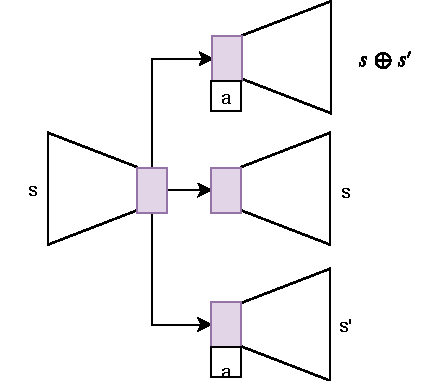
\includegraphics[width=\linewidth]{img/cerberus.pdf}
		\caption{Cerberus}
		\label{subfig:repr_learner_cerberus}
	\end{subfigure}
	\caption{Network architectures of different representation learners, where $s$ and $s'$ indicate current and next state respectively, and $a$ indicates the action leading from $s$ to $s'$. 
	The layers marked in purple are the latent representations to be used as the basis of later transfer learning. 
	The arrows indicate a straight copy from source to target.
	}
	\label{fig:repr_learner}
\end{figure}

\subsubsection{Simple and Variational Autoencoder}
One of the simplest representation learner is an autoencoder, which in our case compresses and reconstructs the current state. %representation. 
Figure \ref{subfig:repr_learner_simple_autoencoder} illustrates the simple autoencoder, and \ref{subfig:repr_learner_vae} a variational autoencoder (VAE). 
%Insert here difference of VAE and AE. 
VAE is a generative approach that models the latent distribution with a Gaussian distribution.
Whether it is simple or variational autoencoder,
one theoretical drawback of using such a simple structure for representation learning is that since the latent space only aims at compressing the state and no dynamics of the task are encoded, it is not necessarily a useful basis for transfer learning.
The upcoming architectures aim to account for this.

\subsubsection{Janus}
To create more guidance in the construction of the latent space, we add another sub-network to capture the dynamics of the environment. 
As shown in Figure \ref{subfig:repr_learner_janus},
in addition to reconstructing the current state, we also append the action in latent space and seek to use this combination to predict the next state.
The hypothesized effect of this approach is that the latent representation is incentivized to preserve transition dynamics in the environment, and therefore is a more meaningful abstraction of the task.

\subsubsection{Cerberus}
Compared to Janus, the Cerberus architecture contains one more output sub-network, which aims to predict the difference between the current and next state. 
By only predicting the differences instead of the next state in its entirety, focus is placed on the change caused by the action taken.
We expect this to be especially useful when the changes between consecutive states are small relative to the entire state representation.
The network architecture is shown in Figure \ref{subfig:repr_learner_cerberus}.  

\subsection{Policy Learners}
Based on the latent space constructed by the representation learner, the policy learner trains an RL agent to complete a given task.
%More specifically, take the output

\subsubsection{Deep Q-Network}
One of the drawbacks of table-based Q-learning occurs in environments with large state spaces.
Maintaining and updating the values of all possible states is memory intensive and requires a great amount of training data.
An alternative that avoids this problem is function approximation. 
We use a Deep Q-Network (DQN) \citep{DQN}, which is a Q-learning algorithm that uses deep neural networks to approximate the state Q-values of each action.

Experience replay is used to improve the learning process in DQN. 
This mechanism stores the situations that the agent previously encountered as ``memories'' and randomly samples them to train the network. 
The sampling of memories is meant to remove correlation between training instances and avoid forgetting previous experiences, facilitating the learning.

Furthermore, prioritized experience replay (PER) \citep{prioritized_memory} was introduced to take into account the loss caused by the memories. With the idea that some experiences are more useful to other to learn, PER weights them with respect to the loss, prioritizing the ones that have a major loss.

%some memory is more important, depending on loss, give more prio to the ones that have major loss. Try to choose the ones causing more loss. 

\subsubsection{Double Deep Q-Network}
Double Deep Q-Network (DDQN) \citep{DDQN} is an improvement to DQN that stabilizes the target Q-values to be predicted. In DQN, the maximization step taken to calculate the next Q-value (Equation \ref{eq:dqn_td}) can lead to inaccurate predictions that generates overestimation bias, affecting the learning process.

\begin{equation}\label{eq:dqn_td}
     Q(s,a) = r(s,a) + \gamma max_{a}Q(s',a)
\end{equation}

By decoupling the selection of the action from the value evaluation, as in equation \ref{eq:ddqn_td}, DDQN addresses this overestimation problem. Two networks are used in this process: the original DQN, used to choose the action that maximizes the Q-value and a target network, $Q_{t}$, that calculates the estimation with the given action.

% This is done by the use of a target network, which will estimate the next Q-value after choosing and action with the DQN network. is updated with the trained network every certain number of steps.

\begin{equation}\label{eq:ddqn_td}
     Q(s,a) = r(s,a) + \gamma Q_{t}(s,argmax_{a}Q(s',a))
\end{equation}

More specifically, the target network is kept fixed for a certain number of steps after which is updated with the DQN weights, that keeps changing every step.

%DQN state, contrary to in DQN where it changes every step.

\iffalse
\begin{itemize}
	\item DDQN  also has prioritized memory 
	%Dueling DQN \citep{DuelingDQN}: state value, mix between q=learning and state action.
	\item DQN update policy every time. 
	\item continuously changing policy, estimate q-value changes every time.
	target network updated every 100 steps. prediction of q-values is fixed. otherwise there is ``more bias''?
\end{itemize}
\fi

\subsection{Parallel Learning}
During training, the agent learns the construction of the latent space and the policy based on the latter  in a parallel approach. In each step of every training episode, first the representation module is trained on a batch of observations. Subsequently, the DDQN is updated based on a state-action-reward-state tuple in which the states were encoded into the latent space using the new version of the representation module. 

\paragraph{Batch Representation Learning} To improve the efficiency of training the representation module, batch learning is used. All observations are stored in memory and are fed into the representation network in minibatches of size 32, randomly sampled from this memory. The memory is limited in its size to 1024 observations and dequeues in a \textit{first-in-first-out} manner.

\paragraph{Full backpropagation} Furthermore, when updating the policy, the loss of the DDQN is also backpropagated through the encoder of the representation module. This additionally biases the representation to be sensible to the collected rewards.\\

A parallel approach to learning the two submodules of the agent implicates that during early episodes, the latent states seen by the DDQN are of very low quality. To counteract this, the training involves a warm up period in which the DDQN learns only on single samples without storing them in a memory. Only after a heuristically chosen amount of steps the replay memory is going to be filled, assuming that the quality of the memories is now sufficient.

\paragraph{Multi-Task Learning} In multi-task learning, the training alters between the tasks by randomly choosing the next environment at the beginning of each episode. If the observations are given to the DDQN in the same order, this could lead to the agent constantly trying to perform well in the new task, instead of finding a general policy. As a solution we propose an experience stack in which each experience (that is, a state-action-reward-state tuple and the done-flag) is stored when observed. After a warm up period that fills the stack, at each step a random element is popped from the stack and fed to the policy.

\paragraph{Intergradient Learning Phases} In the beginning of training, efficient learning of an useful representation is crucial. In later stages, the representation should only be fine-tuned, since the policy needs to see consistent input. Additionally, the training based on the auto-encoder's loss is supposed to guide the encoder towards representing in a generalizable latent space. But when progressing, this guidance should slowly diminish to allow the DDQN to fine-tune the encoder to its own, potentially task-oriented needs. We guarantee such an intergradient learning by introducing a learning rate schedule to the representation module that reduces the learning rate of the auto-encoder by 10 percent every 500 episodes. At the same time the learning rate of the DDQN is kept constant.

\begin{figure}[ht!]
	\centering
	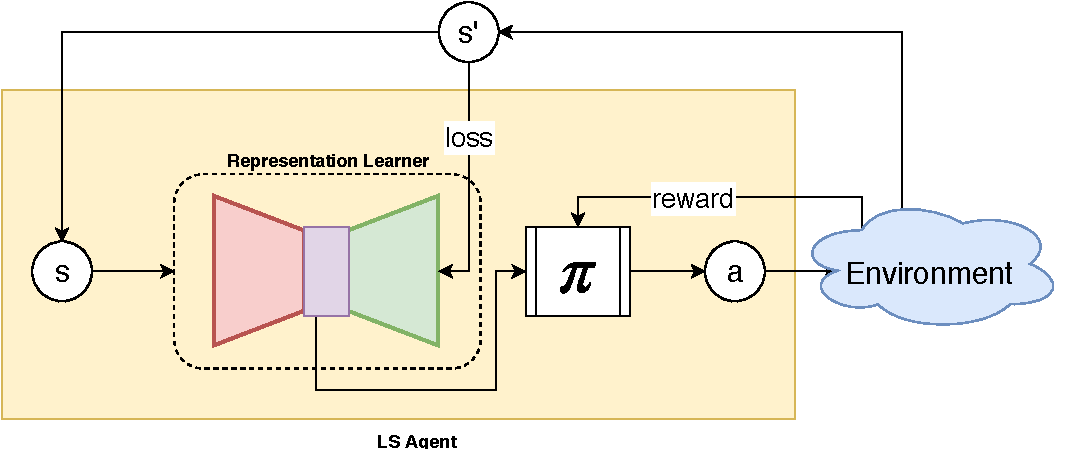
\includegraphics[width=\linewidth]{img/parallel.pdf}
	\caption{Illustration of the parallel approach, where the representation module and policy are trained simultaneously as the agent operates in the environment.\label{fig:approaches}}
\end{figure}

% \subsubsection{History Approach}
% As the name indicates, the history approach first creates a collection of states, actions and rewards by randomly exploring in the environment.
% The representation learner is then trained based on the collected history.
% Once learning completes, the policy learner is trained based on the encoding of the representation learner.
% In this approach, the representation and policy learning are sequential and decoupled. 